\documentclass{article}\usepackage[utf8]{inputenc}\usepackage[T1]{fontenc}\usepackage{lmodern}\usepackage{amsmath}\usepackage{tikz}\pagestyle{empty}\begin{document}\begin{center}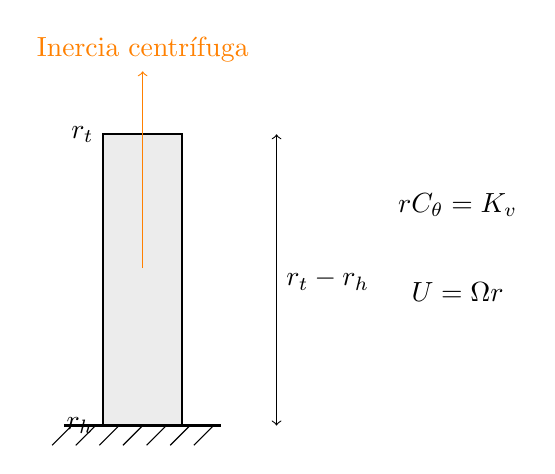
\begin{tikzpicture}\draw[fill=gray!15,thick] (1,0) rectangle (2,3.7);\draw[thick] (.5,0)--(2.5,0);\foreach \x in {.6,.9,...,2.4}{\draw (\x,0)--(\x-.25,-.25);}\draw[->,orange] (1.5,2)--(1.5,4.5) node[above] {Inercia centrífuga};\draw[<->] (3.2,0)--(3.2,3.7) node[midway,right] {$r_t-r_h$};\node[left] at (1,0) {$r_h$};\node[left] at (1,3.7) {$r_t$};\node at (5.5,2.8) {$rC_\theta=K_v$};\node at (5.5,1.7) {$U=\Omega r$};\end{tikzpicture}\end{center}\end{document}